\documentclass[tikz, border=5mm]{standalone}
\usepackage{pgfplots}
\pgfplotsset{compat=1.18}
\usepackage{amsmath}

\begin{document}

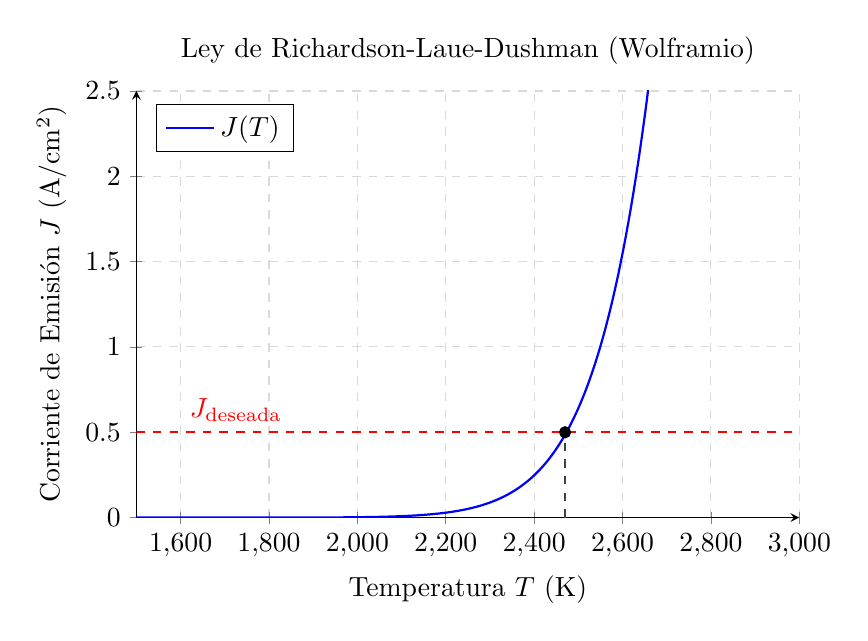
\begin{tikzpicture}
    \begin{axis}[
        width=10cm, height=7cm,
        xlabel={Temperatura $T$ (K)},
        ylabel={Corriente de Emisión $J$ (A/cm$^2$)},
        domain=1500:3000,
        samples=100,
        grid=major,
        grid style={dashed, gray!30},
        axis lines=left,
        title={Ley de Richardson-Laue-Dushman (Wolframio)},
        legend pos=north west,
        scaled y ticks=false,
        ymin=0, ymax=2.5
    ]
        
        % 1. The main Richardson-Laue-Dushman curve
        % Using Tungsten constants: 120 * T^2 * exp(-52200/T)
        \addplot [thick, blue, smooth] {120 * x^2 * exp(-52200/x)};
        \addlegendentry{$J(T)$}

        % 2. Horizontal line: Desired Current (e.g., 0.5 A/cm^2)
        \addplot [thick, red, dashed, domain=1500:3000] {0.5} 
            node[pos=0.15, above, text=red] {$J_{\text{deseada}}$};

        % 3. Vertical line: Ideal Temperature (Intersection at ~2470 K)
        \draw [thick, darkgray, dashed] (axis cs:2470, 0) -- (axis cs:2470, 0.5) 
            node[pos=0, below] {$T_{\text{ideal}}$};
        
        % 4. Intersection Point
        \addplot[mark=*, mark size=2pt, color=black] coordinates {(2470, 0.5)};

    \end{axis}
\end{tikzpicture}

\end{document}